\documentclass[12pt]{article}

\usepackage[T1]{fontenc}
\usepackage[scaled]{beramono}
%\usepackage{bera}
\usepackage{tikz}
\usetikzlibrary{shapes,arrows}
\usepackage{listings}
\usepackage{libertine}
\usepackage[T1]{fontenc}

\usepackage{color}
\definecolor{bluekeywords}{rgb}{0.13,0.13,1}
\definecolor{greencomments}{rgb}{0,0.5,0}
\definecolor{redstrings}{rgb}{0.9,0,0}

\definecolor{mygreen}{rgb}{0,0.6,0}
\definecolor{mygray}{rgb}{0.2,0.2,0.2}
\definecolor{mymauve}{rgb}{0.58,0,0.82}

\usepackage{listings}
\lstset{escapechar=\@}

% Define block styles
\tikzstyle{block} = [rectangle, draw, fill=blue!20, 
    text width=3.2em, text centered, rounded corners, minimum height=3em]
\tikzstyle{line} = [draw, -latex']
    

\title{02242: Program analysis \\ 
		\medskip \large{Technical University of Denmark} \\ \medskip  \large{First draft}}

\author{Ibrahim Nemli - s093477 \\
        Kim Rostgaard Christensen - s084283\\
        Peter Gammelgaard Poulsen - s093263}
\begin{document}
\maketitle
 
\begin{abstract}
This is the report documenting and describing the work done in the course 02242: Program Analysis.
\end{abstract}
\section*{Exercise 1}
For the first exercise we define and discuss the various data structures used for our intermediate representation.
\subsection*{(a) Abstract syntax tree data structure}
%The parser provides a representation of the abstract syntax tree; specify this data structure in your implementation language.
\subsection*{(b) Flow graph data structure}
%Present a data structure for flow graphs and give an algorithms for transforming abstract syntax trees into flow graphs.
This is a typical tree structure, with a parent reference.
\subsection*{(c) Program graph data structure}
Present a data structure for program graphs and give an algorithm for
transforming abstract syntax trees into program graphs.


\section*{**Notes Below**}

\subsection*{Constructing flow graphs}

\begin{description}
   \item[Functions:] Slide 11+12 of from week 2
   \item[label(S):] The set of nodes of the flow graph S
   \item[Init(S):] The initial node of the flow graph S. Unique node where the execution of the program starts.
   \item[Final(S):] The final node of the flow graph S. A set of nodes where the execution of the program may terminate.
   \item[Block(S):] A set of the blocks/statements in the program under inquisition.
   \item[Flow(S):] The edges of the flow graph for S. A set of pairs is returned.
\end{description}

\begin{figure}
\begin{lstlisting}
[y:=x]@$^1$@
[z:=1]@$^2$@
while [x>0]@$^3$@ do
   [z:= z*y]@$^4$@
   [Y:= y-1]@$^5$@
od
[y:=0]@$^6$@
\end{lstlisting}
\label{source:example1}
\caption{Source code example}
\end{figure}

\begin{figure}

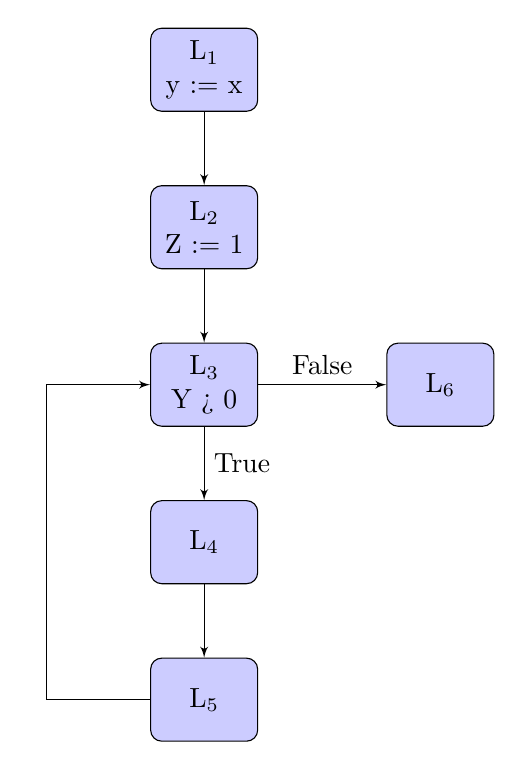
\begin{tikzpicture}[node distance = 2cm, auto]

    % Place nodes
    \node [block] (L1) {L$_1$ \\ y := x};
    \node [block, below of=L1] (L2) {L$_2$ \\ Z := 1};
    \node [block, below of=L2] (L3) {L$_3$ \\ Y > 0};
    \node [block, below of=L3] (L4) {L$_4$ \\ };
    \node [block, below of=L4] (L5) {L$_5$ \\};
    \node [block, right of=L3, node distance=3cm] (L6) {L$_6$ \\};

    % Draw edges
    \path [line] (L1) -- (L2);
    \path [line] (L2) -- (L3);
    \path [line] (L3) -- node {True} (L4);
    \path [line] (L3) -- node {False} (L6);
    \path [line] (L4) -- (L5);
   	\path [line] (L5) -| (-2,-6) |-  node [near start, color=black] {} (L3);

\end{tikzpicture}

\caption{Flow Graph}

\end{figure}

\begin{description}
\item[Label($S$):] $\left\lbrace   1,2,3,4,5,6   \right\rbrace$
\item[Initial($S$):] 1
\item[Final($S$):] $\left\lbrace   6   \right\rbrace$
\item[Blocks($S$):]$\{$ y:=x, z:=1 y>0, z:=z*y, y;=y-1, Y:=0 $\}$
\item[Flow($S$):] $\{ (1,2), (2,3), (3,4), (4,5), (5,3), (3,6) \}$
\end{description}

\subsection*{Constructing program graph}
Functions: Slide 14, week 2.\\
$pg^{qt}_{qs}$: The program graph for statement $S$ with with initial node being $q_{s}$\footnote{$s$ for source.}, and $q_{t}$\footnote{$t$ for target.}\\
Nodes are constructed by the algorithm.\\
The edges are represented by the tuple $(q_s, x, q_T)$ where $q_s$ and $q_t$ are nodes, and x is and elementary block statement. %NOTE, krc: shouldn't x be s ?

\begin{figure}[h]
\centering
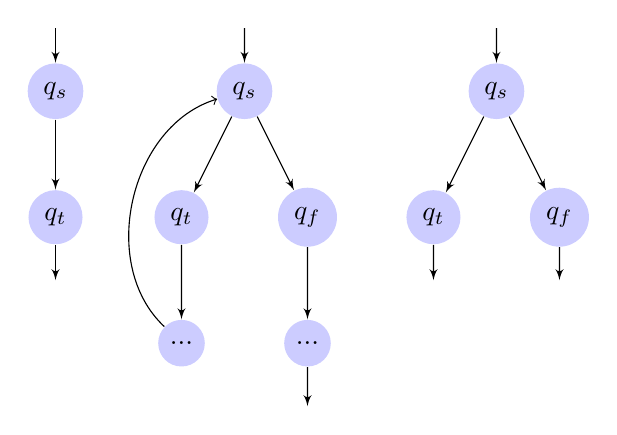
\begin{tikzpicture}
  [scale=.8,auto=left,every node/.style={circle,fill=blue!20}]
  \tikzstyle{line} = [draw, -latex']

  \node (q_s) at (0,3)  {$q_s$};
  \node (q_t) at (0,1)  {$q_t$};

  \path [line] (0,4) -- (q_s);
  \path [line] (q_s) -- (q_t); %TODO; Add label here.
  \path [line] (q_t) -- (0,0);


  \node (q_s) at (3,3)  {$q_s$};
  \node (q_t) at (2,1)  {$q_t$};
  \node (q_f) at (4,1)  {$q_f$};
  \node (empty1) at (2,-1)  {$...$};
  \node (empty2) at (4,-1)  {$...$};

  \path [line] (3,4) -- (q_s);
  \path [line] (q_s) -- (q_t); %TODO; Add label here.
  \path [line] (q_s) -- (q_f); %TODO; Add label here.
  \path [line] (q_f) -- (empty2);
  \path [line] (q_t) -- (empty1);
  \path [line] (empty2) -- (4,-2);
  \draw[bend left=60,->]  (empty1) to (q_s);
  
  \node (q_s) at (7,3)  {$q_s$};
  \node (q_t) at (6,1)  {$q_t$};
  \node (q_f) at (8,1)  {$q_f$};

  \path [line] (7,4) -- (q_s);
  \path [line] (q_s) -- (q_t); %TODO; Add label here.
  \path [line] (q_s) -- (q_f); %TODO; Add label here.
  \path [line] (q_t) -- (6,0);
  \path [line] (q_f) -- (8,0);

\end{tikzpicture}
 \caption{Assignments, loops and branches}

 \label{fig:graph}
\end{figure}

%TODO Figure from 6.jpg

\begin{description}
\item[Label($S$):] $\{ 1,2,3,4,5,6,7 \}$
\item[Initial($S$):] $1$
\item[Final($S$):] $\{ 7 \}$
\item[Blocks($S$):]$\{ [y:=x], [z:=1], [y>0], [z:=z*y], [y;=y-1], [\lnot (y>0)] ,[Y:=0] \}$
\item[Flow($S$):] $\{ (1,2), (2,3), (3,4), (4,5), (5,3), (3,6), (6,7) \}$
\end{description}


\section*{Exercise 2 - Program Slicing}

\subsection*{(a) Example program}
\begin{figure}
\begin{lstlisting}
program
[int x]@$^1$@
[int y]@$^2$@
[int <]@$^3$@
[y := x]@$^4$@
[z := 1]@$^5$@
while [y>0]@$^6$@ do
   [z:= z*y]@$^7$@
   [Y:= y-1]@$^8$@
od
[y:=0]@$^9$@
end
\end{lstlisting}
\label{source:example2}
\caption{Slicing code example}
\end{figure}

The point of interest is label 8.  The result of program slice analysis is; [y:=x]$^4$, [z:=1]$^5$, [z:=z*y]$^7$, [int z]$^3$, [int y]$^2$.\\\\

kill$_{RD}$([int x]$^2$) = $\emptyset$\\
gen$_{RD}$([int x]$^2$) = $\{(x,2)\}$\\\\

kill$_{RD}$([A[n]]$^2$) = $\emptyset$\\
gen$_{RD}$([A[n]$^2$) = $\{(A[0],1), ... (A[i-a],<1)\}$\\


\subsection*{(b) Extending Reaching Definitions Analysis table}
\subsection*{(c) Flow graph}
\subsection*{(d) Program slice calculation algorithm}
\section*{Exercise 3}

\begin{equation}
  \left(L, \mathcal{F}, F, E, \iota, \mathrm{f}.  \right) \frac{1}{x^2}
  \label{eq:hej}
\end{equation}

Where 

\section*{Exercise 4}
\end{document}